% !TeX spellcheck = cs_CZ
{\tikzset{external/prefix={tikz/FYZII/}}
 \tikzset{external/figure name/.add={ch21_}{}}
%---------------------------------------------------------------------------------------------------
% file fey2ch21.tex
%---------------------------------------------------------------------------------------------------
%=========================== Kapitola: Řešení Maxwellových rovnic s proudy a náboji ================
\chapter{Řešení Maxwellových rovnic s proudy a náboji}\label{fyz:IIchaXXI}
\minitoc
  \section{Světlo a elektromagnetické vlny}\label{fyz:IIchaXXIsecI}
  \section{Kulové vlny z bodového náboje}\label{fyz:IIchaXXIsecII}
  \section{Obecné řešení Maxwellových rovnic}\label{fyz:IIchaXXIsecIII}
  \section{Pole oscilujícího dipólu}\label{fyz:IIchaXXIsecIV}
  \section{Potenciály pohybujícího se náboje. Liénardovo a Weichertovo obecné 
  řešení}\label{fyz:IIchaXXIsecV}
  \section{Potenciály náboje pohybujícího se rovnoměrně. Lorentzův vzorec	
  }\label{fyz:IIchaXXIsecVI}
  \section{Příklady a cvičení}\label{fyz:IIchaXXIsecVII}



    \begin{figure}[ht!] %\ref{fyz_fig576}
      \centering
      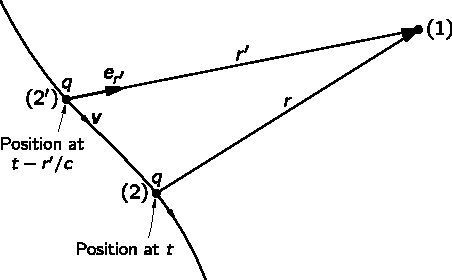
\includegraphics[width=0.7\linewidth]{fyz_fig576.pdf}
      \caption{
               (\cite[s.~707]{Feynman02})}
      \label{fyz_fig576}
    \end{figure}

    \begin{figure}[ht!] %\ref{fyz_fig577}
      \centering
      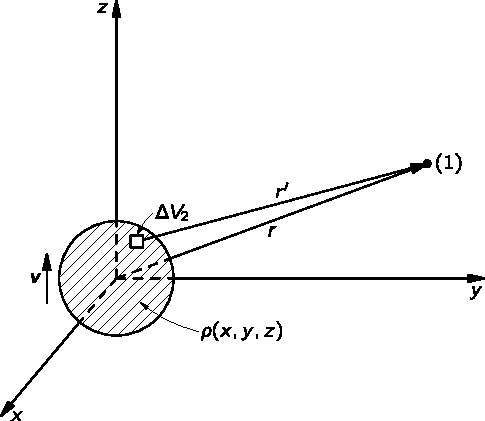
\includegraphics[width=0.7\linewidth]{fyz_fig577.pdf}
      \caption{
               (\cite[s.~707]{Feynman02})}
      \label{fyz_fig577}
    \end{figure}
    
    \begin{figure}[ht!] %\ref{fyz_fig578}
      \centering
      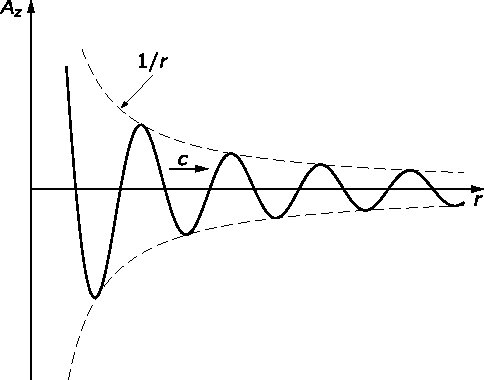
\includegraphics[width=0.7\linewidth]{fyz_fig578.pdf}
      \caption{
               (\cite[s.~707]{Feynman02})}
      \label{fyz_fig578}
    \end{figure}

    \begin{figure}[ht!] %\ref{fyz_fig579}
      \centering
      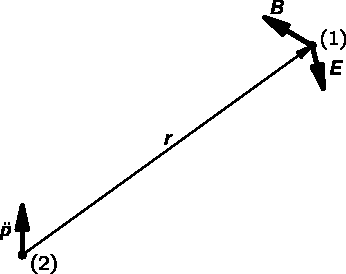
\includegraphics[width=0.7\linewidth]{fyz_fig579.pdf}
      \caption{
               (\cite[s.~707]{Feynman02})}
      \label{fyz_fig579}
    \end{figure}

    \begin{figure}[ht!] %\ref{fyz_fig580}
      \centering
      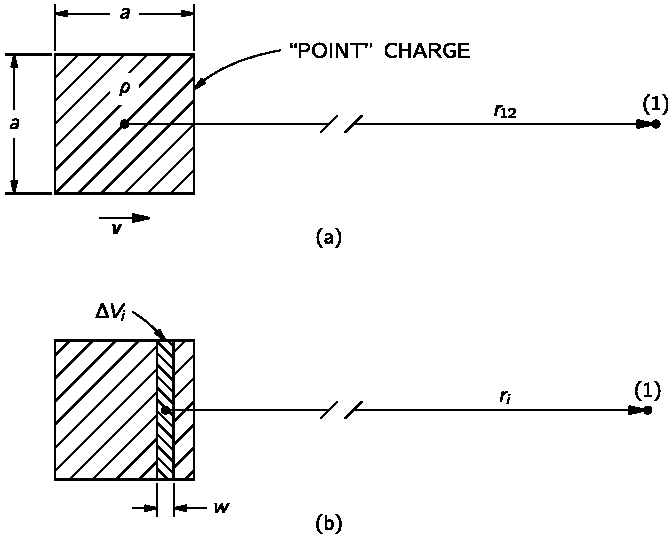
\includegraphics[width=0.7\linewidth]{fyz_fig580.pdf}
      \caption{
               (\cite[s.~707]{Feynman02})}
      \label{fyz_fig580}
    \end{figure}
    
    \begin{figure}[ht!] %\ref{fyz_fig581}
      \centering
      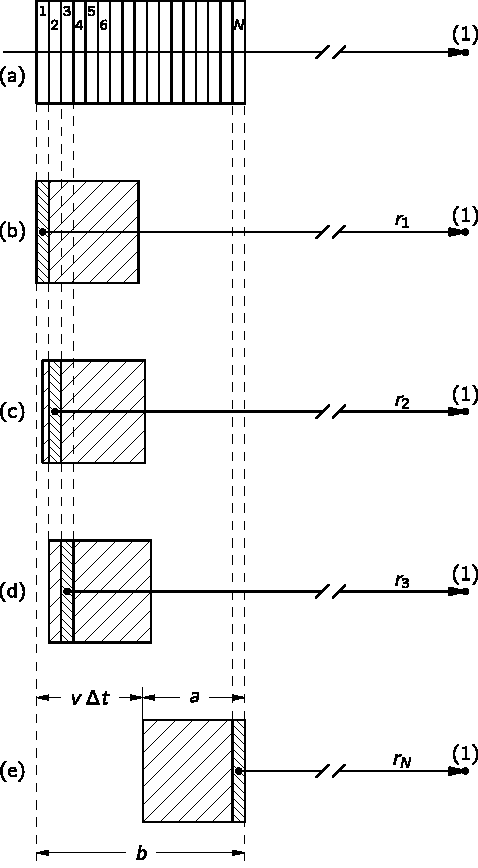
\includegraphics[width=0.7\linewidth]{fyz_fig581.pdf}
      \caption{
               (\cite[s.~707]{Feynman02})}
      \label{fyz_fig581}
    \end{figure}

    \begin{figure}[ht!] %\ref{fyz_fig582}
      \centering
      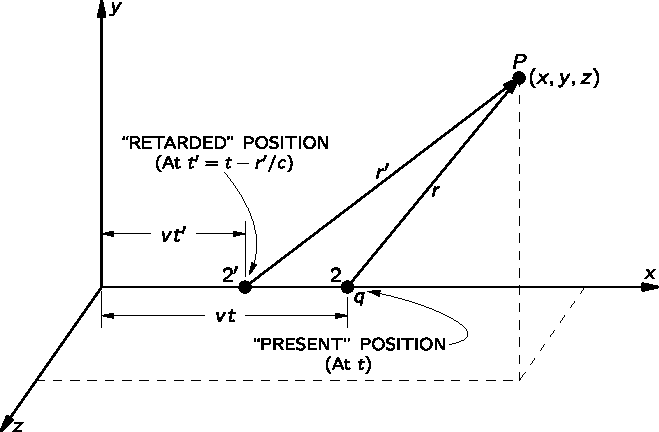
\includegraphics[width=0.7\linewidth]{fyz_fig582.pdf}
      \caption{
               (\cite[s.~707]{Feynman02})}
      \label{fyz_fig582}
    \end{figure}
    
} %tikzset
%---------------------------------------------------------------------------------------------------
%\printbibliography[title={Seznam literatury},heading=subbibliography]
\addcontentsline{toc}{section}{Seznam literatury}